\section{Theorie}

\begin{align*}
    \intertext{Wie beim einfachen Fadenpendel mit der Länge \textbf{l} und der Masse \textbf{m}, wird hier ein reibungsfreier drehbarer Körper mit dem Trägheitsmoment \textbf{I} und mit dem Einfluss des Drehmomentes, 
    aus der Ruhelage, um die Winkel $\phi$ ausgelenkt. Die dabei wirkende Gewichtskraft lautet $ \vec{F} = m \cdot \vec{a} $ und auf den Pendel ausübendes Drehmoments $ M = D_{p} \cdot \phi $. 
    Die Schwingungsgleichung für kleine Auslenkungen und mit dem Trägheitsmoment \textbf{J} ergibt sich}
    J \cdot \ddot{\phi} + D_{p} \cdot \phi = 0. 
    \intertext{Die harmonische Schwingung, die aus der Lösung der Schwingungsgleichung entsteht, hat die Eigenkreisfrequenz} 
    \omega = \sqrt{\frac{D_{p}}{J}} = \sqrt{ \frac{g}{l}}.
    \intertext{Verbindet man zwei gleiche Pendel, z.B. durch eine Feder zu einem Pendel durch zusätzliche Drehmomente. Die enstehende Differentialgleichung}
    J \cdot \ddot{\phi}_{1} + D \cdot \phi_{1} = D_{F} \cdot (\phi_2 - \phi_1) \\
    J \cdot \ddot{\phi}_{2} + D \cdot \phi_{2} = D_{F} \cdot (\phi_1 - \phi_2) 
    \intertext{beschreibt die Schwingung der Pendel sowie die zusätzlich Drehmomente unter Beachtung der Felder.
    Je nach den verschiedenen r Anfangsbedingungen, Variation der Auslenkung, ergeben sich drei Arten von Schwingungen, 
    welche aus Abbildung \ref{Abbildung1} zu entnehmen sind.}  
\end{align*}

\begin{figure}[H] 
    \begin{subfigure}{0.50\textwidth}
        \centering
        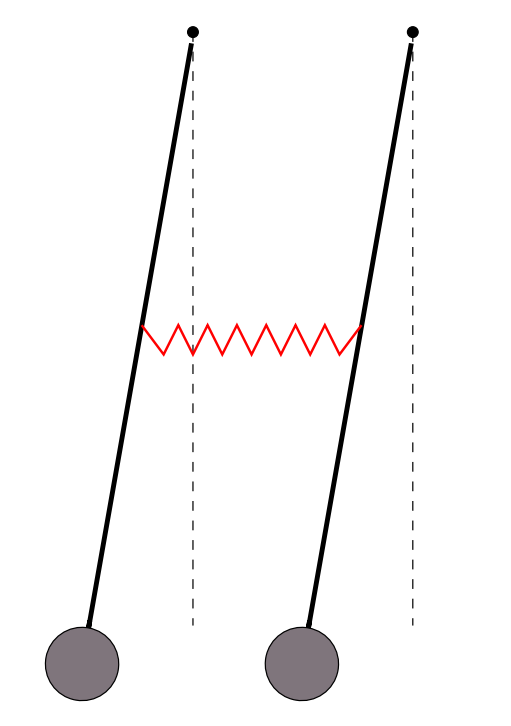
\includegraphics[width=22mm]{bilder/gleichphase.png}
        \caption{Die Abbildung einer gleichsinnigen Schwingung.} 
        \label{Abbildung1a}
    \end{subfigure}
    \hspace{0.3cm}
    \begin{subfigure}{0.50\textwidth}
        \centering
        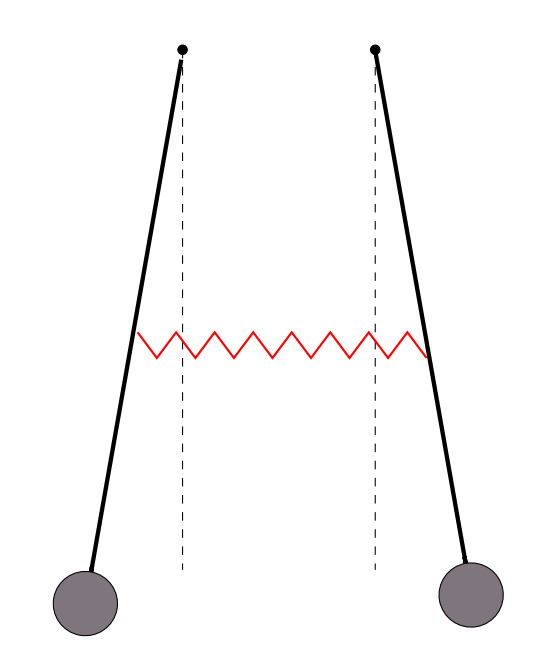
\includegraphics[height=30mm]{bilder/gegenphase.png}
        \caption{Die Abbildung einer gegensinningen Schwingung.} 
        \label{Abbildung1b}
    \end{subfigure}
    \center
    \begin{subfigure}{0.60\textwidth}
        \centering
        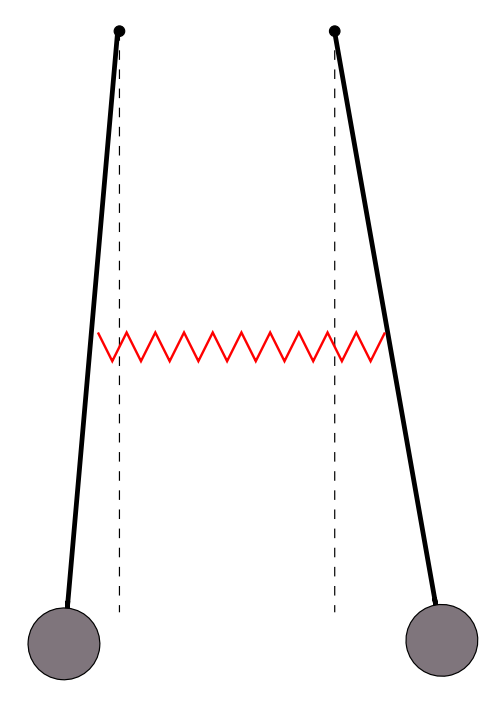
\includegraphics[height=30mm]{bilder/gekoppelte.png}
        \caption{Die Abbildung einer gekoppelten Schwingung.} 
        \label{Abbildung1c}
    \end{subfigure}
    \caption{Die drei im Versuch benötigten Schwingungsabbildungen \cite[2]{aa1}.}
    \label{Abbildung1}
\end{figure}

\begin{flushleft}
    In dem Fall $ \alpha_1 = \alpha_2 $, eine gleichsinnige Schwingung, werden die Pendel um den gleichen Anfangswinkel ausgelenkt.
    Die Pendel schwingen gleichsinnig, ohne dass sich die Feder in ihre Bewegung kaum einwirkt. 
    Dadurch ist ihre Schwingungsfrequenz gleich: 
\end{flushleft}

\begin{align}
    \omega_{+} = \sqrt{\frac{g}{l}} \label{1}
    \intertext{und ihre Schwingungsdauer ebenso:}
    T_{+} = 2\pi \sqrt{\frac{l}{g}}. \label{2}
    \intertext{In dem Fall $ \alpha_{1} = -\alpha_{2} $, eine gegensinninge Schwingung, werden die Pendel um den gleichen Winkelbetrag aber in entgegengesetzte Richtungen ausgelenkt.
    Die Feder übt gegengerichtete Kräfte und Drehmomente aus.
    Es ergibt sich eine symmetrische Schwingung mit der Frequenz} 
    \omega_{-} = \sqrt{ \frac{g}{l} + \frac{2k}{l} } \label{3}
    \intertext{und der Schwingungsdauer}
    T_{-} = 2\pi \cdot \sqrt{\frac{l}{g+2k}} \label{4}
    \intertext{In dem Fall $ \alpha_{1} = 0 $ und $ \alpha_{2} \neq 0 $, eine gekoppel Schwingung, wird ein Pendel in seiner Ruhelage gehalten und das andere um $ \alpha_{2} $ ausgelenkt. 
    Die Energie wird dabei vom ausgelenkten Pendel auf das Ruhende übertragen. 
    Die Amplitude wird somit größer und erreicht sein Maximum, solange die gesamte Energie vom ursprünglich schwingenden Pendel auf das ursprünglich ruhende Pendel übertragen wurde. 
    Der Vorgang kehrt um, bis der Anfangszustand erreicht wird. Die Zeit zwischen den zwei Stillständen wird Schwebung genannt mit: }
    T_{S} = \frac{T_{+} \cdot T_{-} }{T_{+}-T_{-}} \label{5}
    \intertext{und die dazugehörige Frequenz}
    \omega_{S} = \omega_{+} - \omega_{-} \label{6}.
    \intertext{Die Kopplungskonstante \textbf{K} errechnet sich durch} 
    K = \frac{\omega^2_{-} - \omega^2{+}}{\omega^2_{-} + \omega^2_{+}} = \frac{T^2_{+} - T^2_{-}}{T^2_{+} + T^2_{-}} \label{7}.
\end{align}